\documentclass[../main.tex]{subfiles}

\begin{document}

\section{Higgs boson}%
\label{sec:higgs_boson}

\subsection{De noot voor een scalair boson}%
\label{sub:de_noot_voor_een_scalair_boson}

Bekijken we de cross secties van een aantal zelf interacties die kunnen plaatsvinden voor de zwakke interactie bosonen dan zien we bij ongeveer 1TeV dat de unitariteit geschonden wordt, de waarschijnlijkheden voor deze diagrammen worden groter dan 1.

\begin{figure}[h]
    \centering
    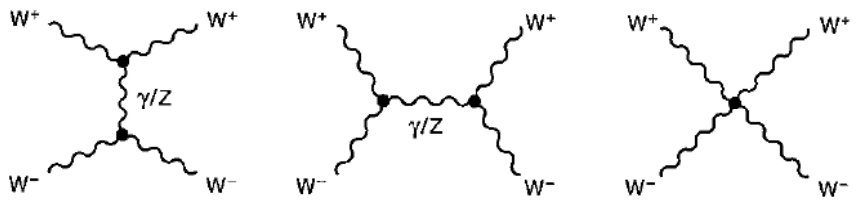
\includegraphics[width=0.8\linewidth]{higgs_boson/zwak_zelf_int_geen_H.png}
    \caption{Mogelijke zelf interactie diagrammen voor het toevoegen van Higgs interacties}%
    \label{fig:higgs_boson/zwak_zelf_int_geen_H}
\end{figure}

Om deze divergenties op te lossen is het nodig om extra parameters toe te voegen. Door het toevoegen van de de koppeling van de $W$ bosonen aan het Higgs boson, een scalair boson, is het mogelijk om de divergentie naar oneindig te convergeren.

\begin{figure}[h]
    \centering
    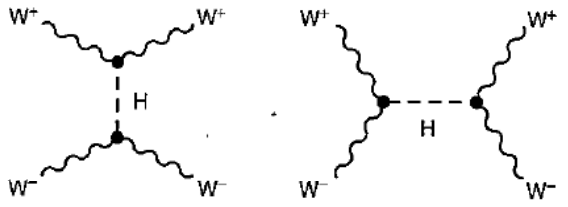
\includegraphics[width=0.6\linewidth]{higgs_boson/zwak_zelf_int_H.png}
    \caption{Toevoegen van Higgs boson interacties}%
    \label{fig:higgs_boson/zwak_zelf_int_H}
\end{figure}

We kunnen aan deze diagrammen direct zien dat de elektrozwakke koppeling van $W$ aan $Z$ een grote invloed zal hebben voor de koppeling van $W$ aan $H$. De opheffing van de divergenties zal enkel werken als de $H$-koppeling gerelateerd is aan de elektrozwakke koppeling.

\subsection{Lagrangiaan}%
\label{sub:lagrangiaan}

Hier moeten we overstappen van het relativistische beeld naar de kwantumvelden theorie omdat Higgs mechanisme en het bestaan van het Higgs boson niet uitgelegd kan worden zonder deze theorie.\\
Klassiek gezien is de Lagrangiaan niets meer dan $L(q_i, \dot{q}_i) = T-V$. Hierbij hoort de klassieke bewegingsvergelijking
\begin{equation}
    \begin{aligned}
        \label{eq:klas_bewegingsvergelijking}
        \frac{d}{dt} \left( \frac{\partial L}{\partial \dot{q}_i} \right) - \frac{\partial L}{\partial q_i} =0
    \end{aligned}
\end{equation}
Wanneer we overschakelen naar veldentheorie worden de plaats en impuls componenten vervangen door veldcoordinaten en zijn afgeleiden, $L(q_i,\dot{q}_i) \rightarrow \mathcal{L}(\phi_i, \partial_\mu\phi_i)$. De bewegingsvergelijking voor de veldentheorie is in essentie gelijk aan de klassieke bewegingsvergelijking.
\begin{equation}
    \begin{aligned}
        \label{eq:velden_bewegingsvergelijking}
        \partial_\mu \left( \frac{\partial \mathcal{L}}{\partial(\partial_\mu \phi_i)} \right) - \frac{\partial \mathcal{L}}{\partial \phi_i} = 0
    \end{aligned}
\end{equation}
In de quantumvelden theorie zijn de deeltjes niet meer dan de kleinste excitaties van de velden, de kwanta. De Lagrangiaan kan nu op verschillende manieren samengesteld worden om verschillende deeltjes te beschrijven. Een aantal voorbeelden hiervan zijn:
\begin{itemize}
    \item Scalair: Deze deeltjes dragen geen spin en pariteit en worden beschreven door
        \begin{equation}
            \begin{aligned}
                \label{eq:lagr_scalair}
                \mathcal{L}_S = \frac{1}{2} (\partial_\mu \phi)(\partial^\mu \phi) = \frac{1}{2} m^2\phi^2
            \end{aligned}
        \end{equation}
        De veldfuncties $\phi$ die door deze Lagrangiaan beschreven worden voldoen aan de Klein-Gordon vergelijkingen. De kwanta hiervan zijn Higgs bosonen.
    \item Dirac: Dirac deeltjes worden beschreven door
        \begin{equation}
            \begin{aligned}
                \label{eq:lagr_dirac}
                \mathcal{L}_D = i\overline \psi \gamma^\mu \partial_\mu \psi - m \overline \psi\psi
            \end{aligned}
        \end{equation}
        De veldgolffuncties voldoen hier natuurlijk aan de Dirac vergelijking en zijn dus 4 vectoren met als kwanta de fermionen.
        \begin{equation}
            \begin{aligned}
                \label{eq:veld_func_dirac}
                \psi(x) =
                \begin{pmatrix}
                    \psi_1\\
                    \psi_2\\
                    \psi_3\\
                    \psi_4\\
                \end{pmatrix}=
                \begin{pmatrix}
                    \Psi_1 + i\Phi_1\\
                    \Psi_2 + i\Phi_2\\
                    \Psi_3 + i\Phi_3\\
                    \Psi_4 + i\Phi_4\\
                \end{pmatrix}
            \end{aligned}
        \end{equation}
    \item Vector: Ten laatste wordt de vector Lagrangiaan gegeven door
        \begin{equation}
            \begin{aligned}
                \label{eq:lagr_vec}
                \mathcal{L}_{EM} = - \frac{1}{4} F^{\mu\nu}F_{\mu\nu}
            \end{aligned}
        \end{equation}
        Deze veldfuncties $F_{\mu\nu}$ volgen de Maxwell vergelijkingen en kunnen neergescheven worden als
        \begin{equation}
            \begin{aligned}
                \label{eq:veld_func_em}
                f^{\mu\nu} = \partial^\mu A^\nu - \partial^\nu A^\mu =
                \begin{pmatrix}
                    0 & -E_x & -E_y & -E_z \\
                    E_x & 0 & -B_z & B_y \\
                    E_y & B_z & 0 -B_x \\
                    E_z & -B_y & B_x & 0 \\
                \end{pmatrix}
            \end{aligned}
        \end{equation}
        De kwanta van dit veld zijn fotonen.
\end{itemize}

\subsection{Lakale $U(1)$ ijk(=gauge) invariantie}%
\label{sub:lakale_u_1_gauge_invariantie}

Als we eisen dat de Lagrangiaan invariant moet zijn onder $\psi(x) \rightarrow \psi'(x) = e^{iq\chi(x)}\psi(x)$. Dit is niets anders dan de fase overal te gaan veranderen of dit kan ook gezien worden als een rotatie in de ruimte met hoek $\chi(x)$. De ruimte afhankelijkheid van de hoek slaat neet op het lokale gedeelte van de invariantie. Bijvoorbeeld voor de Dirac Lagrangiaan krijgen we dan
\begin{equation}
    \begin{aligned}
        \label{eq:lok_ijk_inv_dir_1}
        \mathcal{L} &= i\overline \psi \gamma^\mu \partial_\mu \psi - m \overline \psi\psi\\
        \mathcal{L} \rightarrow \mathcal{L}' &= i e^{-iq\chi} \overline \psi \gamma^\mu [e^{iq\chi}\partial_\mu \psi + iq(\partial_\mu\chi) e^{iq\chi}\psi] - m e^{iq\chi} \overline \psi e^{iq\chi}\psi\\
                                             &=\mathcal{L} - q\overline \psi \gamma^\mu (\partial_\mu \chi)\psi
    \end{aligned}
\end{equation}
Om deze extra term weg te werken en de invariantie te eisen is door over te gaan op een covariante afgeleide $D_\mu$ waar een extra veld $A_\mu$ in verwerkt zit.
\begin{equation}
    \begin{aligned}
        \label{eq:cov_afgeleide}
        \partial_\mu &\rightarrow D_\mu = \partial_\mu + iqA_\mu\\
        A_\mu &\rightarrow A'_\mu = A_\mu - \partial_\mu \chi
    \end{aligned}
\end{equation}
Hierdoor krijgen we een nieuwe ijk invariante Lagrangiaan:
\begin{equation}
    \begin{aligned}
        \label{eq:lok_ijk_inv_dir_2}
        \mathcal{L} = \overline \psi (i\gamma^\mu \partial_\mu - m)\psi - q\overline\psi\gamma^\mu A_\mu\psi
    \end{aligned}
\end{equation}
Wat er hier dus gebeurd is, is dat de lokale informatie van $\chi$ moet doorgegeven kunnen worden aan de rest van het veld. Dit moet ingebakken zijn in de Lagrangiaan. Dit wordt gedaan door te koppelen aan het veld $A_\mu$ waar die informatie van de fase in zit. De sterke waarmee $\psi$ aan $A$ zal koppelen is $q$.\\
Bij het opleggen van de lokale ijk invariantie gebeuren er 2 dingen. Er ontstaat een veld die informatie bevat over de lokale ijk en het veld moet kunnen koppelen met lading $q$. Dit zal ertoe leiden dat de lading (bv. elektromagnetische, kleur, zwakke lading) moet behouden worden.\\ 
Om te weten hoe het veld $A$ transformeert moeten we nog 1 term toevoegen aan de Lagrangiaan, de elektromagnetische Lagrangiaan.
\begin{equation}
    \begin{aligned}
        \label{eq:lok_ijk_inv_qed}
        \mathcal{L} = \overline \psi (i\gamma^\mu \partial_\mu - m)\psi {\color{red}- q\overline\psi\gamma^\mu A_\mu\psi} {\color{green}- \frac{1}{4} F_{\mu\nu}F^{\mu\nu}}
    \end{aligned}
\end{equation}
De betekenis van de 3 termen in de QED Lagrangiaan zijn in het zwart de beschrijving van de deeltjes, in het groen de beschrijving van het veld en in het groen de interactie tussen de deeltjes en het veld.

\subsection{Massa van de deeltjes}%
\label{sub:massa_van_de_deeltjes}

Laten we nu ook massa geven aan dat ijkveld dat we daarjuist hebben ingevoerd. Dit kan gedaan worden door een massa term aan de Lagrangiaan toe te voegen.
\begin{equation}
    \begin{aligned}
        \label{eq:qed_lagr_met_massa}
        \mathcal{L}_{QED} = \overline \psi (i\gamma^\mu \partial_\mu - m)\psi - q\overline\psi\gamma^\mu A_\mu\psi - \frac{1}{4} F_{\mu\nu}F^{\mu\nu} + \frac{1}{2} m_\gamma^2 A_\mu A^\mu
    \end{aligned}
\end{equation}
Wat hier opvalt is dat bosonen in hun massaterm een $m^2$ hebben staan en de fermionen maar een $m$. De reden hiervoor was dat er problemen waren bij die kwadratische term voor spin $1/2$ deeltjes. Voeren we nu de lokale ijk transformatie uit op deze term
\begin{equation}
    \begin{aligned}
        \label{eq:lok_ijk_tran_massa_term}
        \frac{1}{2} \rightarrow \frac{1}{2} m_\gamma^2(A_\mu-\partial_\mu\chi)(A_\mu-\partial_\mu\chi) \neq \frac{1}{2} m_\gamma^2 A_\mu A^\mu
    \end{aligned}
\end{equation}
We zien dat het ijk boson massaloos moet zijn om te voldoen aan de lokale ijk transformaties. Het massaloos zijn van het foton is een simpel voorbeeld van het Goldstone theorema. Dit theorema zegt dat voor eender welke lokale ijk invariantie je eist moeten de ijkbosonen van deze velden massaloos zijn. Wat nu met de $SU(2)$ theorie? Deze heeft ijkbosonen die een massa hebben wat botst met dit theorema.

\subsection{Interagerende scalaire velden}%
\label{sub:interagerende_scalaire_velden}

Om dit probleem van de massaloze bosonen aan te pakken wordt er gekeken naar een scaleir veld met potentiaal $V(\phi) = \frac{1}{2}\mu^2\phi^2+\frac{1}{4}\lambda\phi^4$. De Lagrangiaan is dus
\begin{equation}
    \begin{aligned}
        \label{eq:lagr_hoed_pot}
        \mathcal{L} = \frac{1}{2} (\partial_\mu \phi) (\partial^\mu \phi) - \frac{1}{2} \mu^2 \phi^2 - \frac{1}{4} \lambda \phi^4
    \end{aligned}
\end{equation}
Indien dat $\lambda$ kleiner is dan 0 is er geen minimum. $\lambda$ moet groter dan 0 zijn. Nemen we nu $\mu^2>0$ dan is de eerste term van de Lagrangiaan de kinetische energie van het deeltje, de tweede de massa van het deeltje en de laatste term de zelf interactie term van het veld.\newpage

\begin{figure}[h]
    \centering
    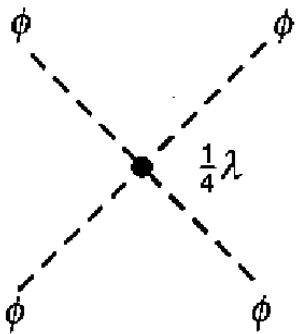
\includegraphics[width=0.2\linewidth]{higgs_boson/zelf_int_term_scal.png}
    \caption{Feynman diagram van de zelf interactie van het scalaire veld}%
    \label{fig:higgs_boson/zelf_int_term_scal}
\end{figure}

De potentiaal heeft enkel een minimum in $\phi=0$.

\begin{figure}[h]
    \centering
    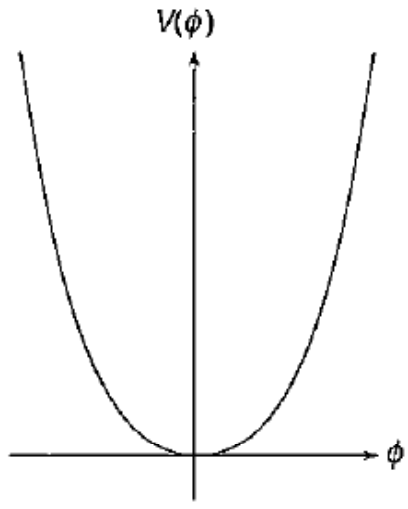
\includegraphics[width=0.2\linewidth]{higgs_boson/hoed_pot_1.png}
    \caption{De hoed potentiaal met $\mu^2>0$}%
    \label{fig:higgs_boson/hoed_pot_1}
\end{figure}

Nemen we nu $\nu^2<0$ krijgen we nu 2 minima in de potentiaal bij $\pm v$.

\begin{figure}[h]
    \centering
    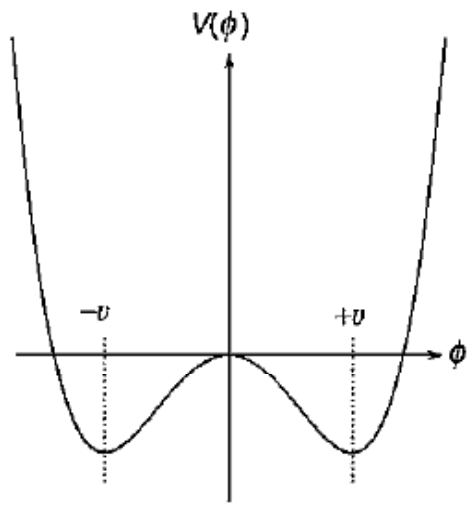
\includegraphics[width=0.2\linewidth]{higgs_boson/hoed_pot_2.png}
    \caption{De hoed potentiaal met $\mu^2<0$}%
    \label{fig:higgs_boson/hoed_pot_2}
\end{figure}

De tweede term is nu geen massaterm meer en hebben we een massaloos deeltje dat beweegt in een bepaalde potentiaal. De vacuum toestand wat de laagste toestand is ligt bij $\phi = \pm v = \pm \left| \sqrt{ \frac{-\mu^2}{\lambda}} \right|$. Dit is nu juist waar de symmetrie wordt gebroken. Nemen we nu de vacuum toestand bij $\phi = +v$ (hier maken we een verschil tussen $\pm v$ en breken we de symmetrie) is het mogelijk om $\phi$ te herschrijven.
\begin{equation}
    \begin{aligned}
        \label{eq:veld_symm_breking}
        \phi(x) &= v+\eta(x)
    \end{aligned}
\end{equation}
$eta$ is hier de beschrijving van het deeltje in de put (hoeveel deze dus afwijkt van $v$). Vullen we dit in in vergelijking (\ref{eq:lagr_hoed_pot}) geeft het volgende
\begin{equation}
    \begin{aligned}
        \label{eq:lagr_hoed_pot_symm_breking}
        \mathcal{L} &= \frac{1}{2} (\partial_\mu \eta) (\partial^\mu \eta) - \frac{1}{2} \mu^2 (v+\eta)^2 - \frac{1}{4} \lambda (v+\eta)^4\\
                    &\downarrow \mu^2= v^2\lambda\\
        &= \frac{1}{2} (\partial_\mu \eta) (\partial^\mu \eta) - \lambda v^2\eta^2 - \lambda v \eta^4 - \frac{1}{4} \lambda \eta^4 + \frac{1}{4} \lambda v^4\\
    \end{aligned}
\end{equation}
Wat we nu kunnen zien is een massief scalair veld met $m_\eta = \sqrt{2\lambda v^2}  \sqrt{-2\nu^5}$ met 2 self interacties van het $\eta$ veld.

\begin{figure}[h]
    \centering
    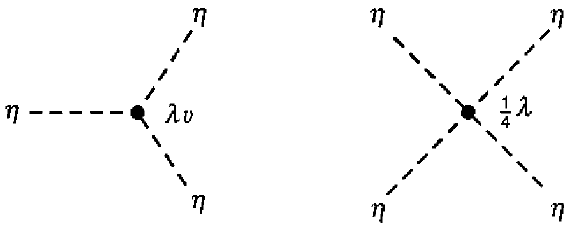
\includegraphics[width=0.4\linewidth]{higgs_boson/zelf_int_eta.png}
    \caption{Zelf interacties van het $\eta$ veld}%
    \label{fig:higgs_boson/zelf_int_eta}
\end{figure}

De laatste term in de Lagrangiaan is een constante en omdat de Lagrangiaan altijd in afgeleides voorkomt in bewegingsvergelijking is deze term niet relevant.

\subsection{Complexe scalaire velden}%
\label{sub:complexe_scalaire_velden}

Introduceren we de nu het complexe scalaire veld en de Lagrangiaan dat dat hierbij hoort.
\begin{equation}
    \begin{aligned}
        \label{eq:complex_scalair_veld}
        \phi &= \frac{1}{\sqrt{2}} (\phi_1 + i\phi_2)\\
        \mathcal{L} &= (\partial_\mu \phi)^*(\partial^\mu\phi) - \mu^2(\phi^*\phi) - \lambda(\phi^*\phi)^2
    \end{aligned}
\end{equation}
De hoed potentiaal zal in deze omstandigheden geroteerd worden rond de as loodrecht op het $\phi_1\phi_2$ vlak.

\begin{figure}[h]
    \centering
    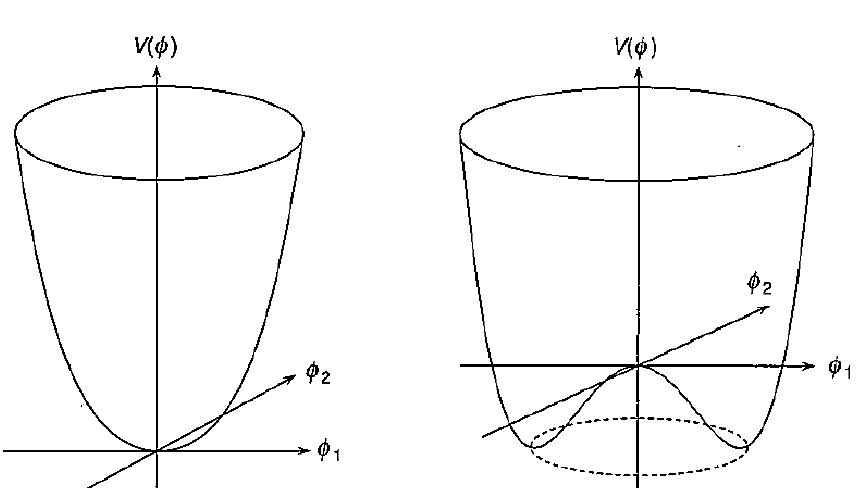
\includegraphics[width=0.6\linewidth]{higgs_boson/hoed_pot_comp.png}
    \caption{Complexe uitbreiding van de hoed potentiaal}%
    \label{fig:higgs_boson/hoed_pot_comp}
\end{figure}

Deze zal in dit geval invariant zijn onder de globale $U(1)$ transformatie $\phi \rightarrow e^{i\alpha}\phi$. Voor $\nu^2<0$ krijgen we nu een ring van minima bij
\begin{equation}
    \begin{aligned}
        \label{eq:complex_symm_breking}
        \phi_1^2+\phi_2^2 = -\frac{\mu^2}{\lambda} =v^2
    \end{aligned}
\end{equation}
We kiezen de vacuum toestand bij $(\phi_1, \phi_2) = (v,0)$ wat de globale $U(1)$ symmetrie spontaan zal breken. Expanderen we deze vacuum toestand en vullen we deze in de Lagrangiaan in dan krijgen we uiteindelijk:
\begin{equation}
    \begin{aligned}
        \label{eq:comple_scalair_veld_symm_breking}
        \phi_1(x) &= \eta(x) + v\\
        \phi_2(x) &= \xi(x)\\
        \mathcal{L} &= \frac{1}{2} (\partial_\nu \eta) (\partial^\mu \eta) + \frac{1}{2} (\partial_\nu \xi) (\partial^\mu \xi) - V(\eta, \xi)\\
        V(\eta, \xi) &= -\frac{1}{4} \lambda v^4 + \lambda v^2 \eta^2 + \lambda v \eta^3 + \frac{1}{4} \lambda \eta^4 + \frac{1}{4} \lambda \xi^4 + \lambda v \eta\xi^2 + \frac{1}{2} \lambda \eta^2\xi^2
    \end{aligned}
\end{equation}
Uit al deze termen kunnen we een aantal elementen waarnemen. Er is een scalair veld aanwezig met massa $m_\eta = \sqrt{2\lambda v^2}$ en een massaloos scalair veld $\xi$. Zoals te zien in de potentiaal kunnen deze 2 velden aan zelf interacties doen. Deze interacties komen overeen met de volgende diagrammen.

\begin{figure}[h]
    \centering
    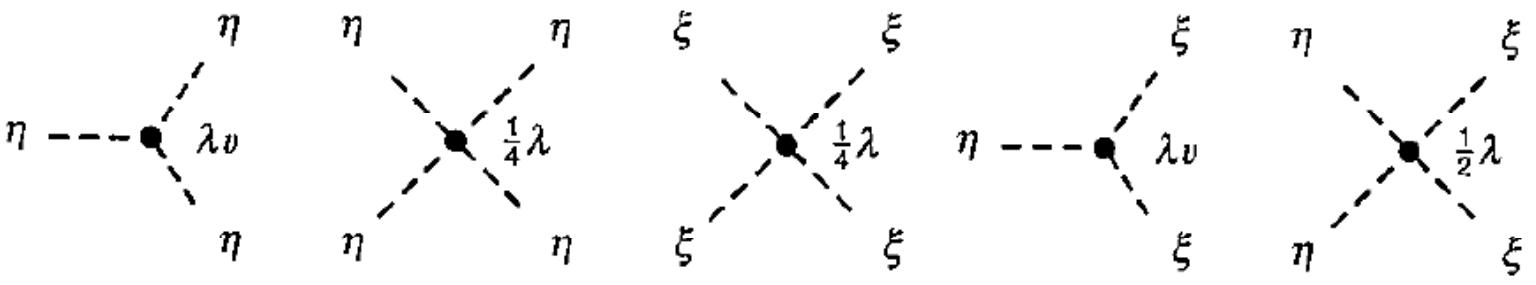
\includegraphics[width=0.8\linewidth]{higgs_boson/complex_scalair_veld_int.png}
    \caption{Zelf interactie diagrammen van complex scalair veld}%
    \label{fig:higgs_boson/complex_scalair_veld_int}
\end{figure}

Het massaloze deeltje komt overeen met de perturbatie van het deeltje langs de cirkel van minima. Om zich hierlangs te verplaatsen is er geen extra energie nodig en wil dit dus zeggen dat het massaloos is.

\subsubsection{Lokale ijk symmetrie}%
\label{ssub:lokale_ijk_symmetrie}

Gaan we nu over van de globale symmetrie naar de lokale $U(1)$ symmetrie moeten we de covariante afgeleide terug invoeren.
\begin{equation}
    \begin{aligned}
        \label{eq:complex_scalair_veld_lokaal}
        \phi(x) &\rightarrow \phi'(x) = e^{ig\chi(x)}\phi(x)\\
        \partial_\mu &\rightarrow D_\mu = \partial_\mu + igB_\mu\\
        B_\mu &\rightarrow B'_\mu = B_\mu - \partial_\mu \chi(x)
    \end{aligned}
\end{equation}
We voeren hier in essentie hetzelfde uit als sectie \ref{sub:lakale_u_1_gauge_invariantie} maar dan voor deeltjes met een andere potentiaal. Hierbij hebben we bij het vervangen van de afgeleide door een de covariante afgeleide terug een extra vector veld $B_\mu$ toegevoegd die de informatie zal dragen van de lokale fases. De Lagrangiaan wordt nu
\begin{equation}
    \begin{aligned}
        \label{eq:comp_scal_veld_lagr_lok_symm}
        \mathcal{L} = - \frac{1}{4} F^{\mu\nu}F^{\mu\nu} + (\partial_\mu \phi)^*(\partial^\mu \phi)-\mu^2\phi^2-\lambda\phi^4\\
        - igB\mu \phi^* (\partial^\mu \phi) + ig (\partial_\mu \phi)^* B^\mu \phi + g^2 B_\mu B^\mu \phi^* \phi
    \end{aligned}
\end{equation}
Hier krijgen we terug een aantal extra termen in de Lagrangiaan. We zien dat een massaloos ijkveld $F^{\mu\nu} = \partial^\mu B^\nu - \partial^\nu B^\mu$ is toegevoegd. De derde laatste toont ook dat dit massaloos ijkveld zal interageren met $\phi$. Werken we de symmetrie breking bij $\mu^2<0$ uit met $\phi(x)= \frac{1}{\sqrt{2}} (v + \eta(x) + i\xi(x))$ vinden we een nieuwe Lagrangiaan
\begin{equation}
    \begin{aligned}
        \label{eq:comp_scal_veld_lagr_lok_symm_breking}
        \mathcal{L} = {\color{red}\frac{1}{2} (\partial_\nu\eta)(\partial^\nu\eta) + \lambda v^2\eta^2} + {\color{blue}\frac{1}{2} (\partial_\nu\xi)(\partial^\nu\xi)} - {\color{green}V_{int}(\eta,\xi,B)}\\
        - {\color{orange}\frac{1}{4} F^{\mu\nu}F_{\mu\nu} + \frac{1}{2} g^2v^2B_\mu B^\mu} + {\color{purple}gvB_\mu(\partial^\mu \xi)}
    \end{aligned}
\end{equation}
In het rood vinden we de beschrijving van het scalair veld $\eta$ dat massief is geworden, in het blauw een massaloos scalaire veld $\xi$, in het groen de interacties tussen $\eta$, $\xi$ en $B$, in oranje het massieve B veld en ten laatste in het paars een directe koppeling van het $B$ veld met het $\xi$ veld. Maar wat is de laatste term nu? Deze klopt niet echt. Het is mogelijk om van deze term af te geraken door een specifieke ijk te kiezen en van daar alles te interpreteren. De ijk die we hier opleggen noemen we de unitaire ijk, $\chi(x) = -\xi(x)/gv$. De complexe term van de golffunctie wordt door deze ijk opgenomen door $v$ en geeft $\phi(x) = \frac{1}{\sqrt{2}} (v+\eta(x)) \equiv \frac{1}{\sqrt{2}} (v+h(x))$. Hierdoor komt $\xi(x)$ niet meer expliciet voor in de Lagrangiaan maar deze zal wel voorkomen in de transformaties $B_\mu (x) \rightarrow B'_\mu(x) - B_\mu(x) + \frac{1}{gv} \partial_\mu \xi(x)$.
\begin{equation}
    \begin{aligned}
        \label{eq:comp_scal_veld_lagr_unitaire_ijk}
        \mathcal{L} = \frac{1}{2} (\partial_\nu h)(\partial^\nu h) + \lambda v^2 h^2 + \frac{1}{2} (\partial_\nu\xi)(\partial^\nu\xi) - \frac{1}{4} F^{\mu\nu}F_{\mu\nu} + \frac{1}{2} g^2v^2B_\mu B^\mu\\
        + gvB_\mu(\partial^\mu h) + \frac{1}{2} g^2 B_\mu B^\mu h^2 - \lambda vh^3 - \frac{1}{4} \lambda h^4
    \end{aligned}
\end{equation}
Hierbij zijn de $\eta$ termen vervangen door Higgs termen. We hebben nog steeds het $B$ veld en de directe koppeling van $B$ en $\xi$ is verdwenen. De $\xi$ termen zijn als het ware opgeslokt door het $B$ veld. Zo bekomen we een Lagrangiaan die 2 massieve velden beschrijft met hun inderlinge interacties daarbij. De massa van deze velden zijn $m_B = gv$ en $m_h = \sqrt{2\lambda}v$.

\begin{figure}[h]
    \centering
    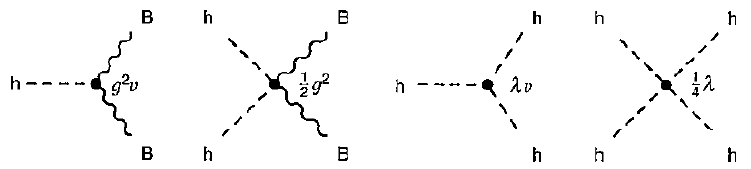
\includegraphics[width=0.8\linewidth]{higgs_boson/complex_scal_int_unitaire_ijk.png}
    \caption{Interactie diagrammen van de velden bij de unitaire ijk}%
    \label{fig:higgs_boson/complex_scal_int_unitaire_ijk}
\end{figure}

\subsection{Het standaard model scalair}%
\label{sub:het_standaard_model_scalair}

In het standaard model hebben we natuurlijk niet alleen lokale $U(1)$ ijk symmetrie maar hebben we eerder een lokale $SU(2)_L\times U(1)_Y$ ijk symmetrie. Deze zullen opbreken in 3 massieve velden $W^+$, $W^-$ en $Z$. Om dit te doen hebben we een scalair veld nodig met 4 vrijheidsgraden.
\begin{equation}
    \begin{aligned}
        \label{eq:sm_scalair_veld}
        \phi = 
        \begin{pmatrix}
            \phi^+\\
            \phi^-
        \end{pmatrix}
        = \frac{1}{\sqrt{2}} 
        \begin{pmatrix}
            \phi_1 + i\phi_2\\
            \phi_3 + i\phi_4
        \end{pmatrix}
    \end{aligned}
\end{equation}
Indien je dit helemaal zou uitwerken (zie Thomson) kan je de verschillende massa's voor de deeltjes: $m_W = \frac{1}{2} gv$, $m_A = 0$, $m_Z = \frac{1}{2} v\sqrt{g^2+g'^2}$ en $m_h = \sqrt{2\lambda}v$. Uit experimenten is het mogelijk om de massa's van deze deeltjes te bepalen en is het mogelijk om andere parameters te berekenen. Zo komt uit $m_W$ en $g$ dat het vacuum $v=246$GeV is. De reden hiervoor weten we niet. Uit $m_W$ en $m_Z$ kunnen we zoals we eerder al gezien hebben de Weinberg hoek $\theta_W$ bepalen. Het was uit de theorie nog niet mogelijk om de massa van het Higgs boson te bepalen omdat er nog een onbekende $\lambda$ was.

\begin{figure}[h]
    \centering
    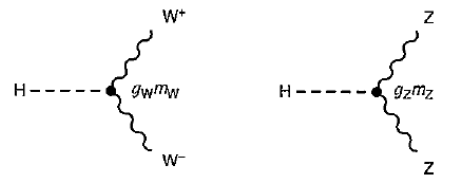
\includegraphics[width=0.6\linewidth]{higgs_boson/koppeling_higgs_wz_boson.png}
    \caption{Koppeling van $W$ en $Z$ aan het Higgs veld}%
    \label{fig:higgs_boson/koppeling_higgs_wz_boson}
\end{figure}

Voor de koppelingsconstante van deze deeltjes hebben we $g_W=g$, $g_Z= \frac{g}{\cos\theta_W}$ en zien we dat de koppeling van het $W$ en $Z$ boson aan het Higgs veld zullen afhangen van hun massa.\\
{\color{red} Het is hier niet de bedoeling om de Lagrangianen volledig te kunnen afleiden op het examen zoals hier is gedaan, het is veel belangrijker om de Lagrangianen te kunnen interpreteren en er de fysische betekenissen van kunnen geven.}

\subsection{Fermion massa's}%
\label{sub:fermion_massa_s}

\begin{figure}[h]
    \centering
    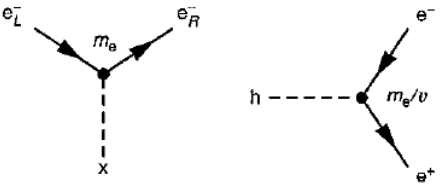
\includegraphics[width=0.6\linewidth]{higgs_boson/koppeling_higgs_e.png}
    \caption{Koppeling van fermionen aan het Higgs veld}%
    \label{fig:higgs_boson/koppeling_higgs_e}
\end{figure}

Zoals de $W$ en $Z$ bosonen krijgen de fermionen ook massa door te koppelen aan het Higgs boson. De koppelingsconstante tussen deze 2 is gegeven door $g_f = \sqrt{2} \frac{m_f}{v} = \frac{m_f}{\sqrt{2}m_W} g$. Deze koppelingen zitten echter niet verwerkt in het Standaard Model. Deze moeten gemeten worden:
\begin{equation}
    \begin{aligned}
        \label{eq:kc_h_fermionen}
        g_t &= 0.997 \pm 0.006\\
        g_e &\approx 3\cdot 10^{-6}\\
        g_\nu &\leq 10^{-12}
    \end{aligned}
\end{equation}
Vroeger was de vraag waarom de top quark zo zwaar was. Dit is eigenlijk de normaal en moeten we ons af vragen waarom de andere fermionen zo licht koppelen aan het Higgs veld.

\end{document}
